\documentclass[../main.tex]{subfiles} % required, if the Chapter be a seperate doc

\begin{document}
\section{Zusammenfassende Tabellen}\label{sec:zusammenfassende-tabellen}
    \subsection{Tabellen}\label{subsec:tabellen}
    \begin{figure}[H]
        \centering
        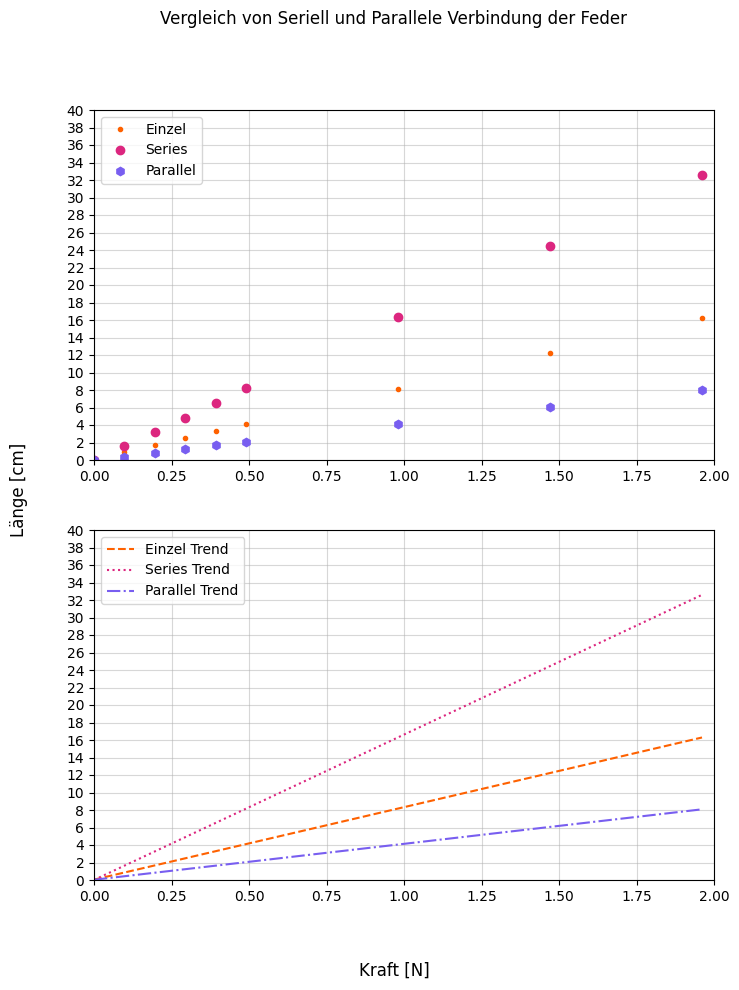
\includegraphics[scale=0.6]{graph/Spring-setup-comparison}
        \caption{Die Darstellung der Feder Positionen einzeln, in Seriell und in Parallel mit Datenpunkte und Trendlinien}\label{fig:figure}
    \end{figure}
    \section{Resultat}\label{subsec:resultat}
    \text{Das Resultat unseres Experiments ist, dass die Feder konstante 0.1209 N/cm beträgt..}

\end{document}
